\documentclass{article}
\usepackage[T1]{fontenc}
\usepackage{lmodern}
\usepackage{graphicx}
\usepackage{amsmath,amssymb}
\usepackage[a4paper,margin=2cm]{geometry}
\usepackage[absolute,overlay]{textpos}
\setlength{\TPHorizModule}{1mm}
\setlength{\TPVertModule}{1mm}
\usepackage[indonesian]{babel}
\usepackage{hyperref}
\setlength{\emergencystretch}{2em}
% unit: Halaman 6

\begin{document}

% === Halaman 6 (llm) ===

\begin{center}
\Huge Hybrid Cryptography
\end{center}

\vspace{100mm}

\noindent \url{https://www.researchgate.net/figure/Illustration-of-a-hybrid-cryptosystem_fig8_327799148}

\vspace{5mm}

\noindent Rinaldi M/II4020 Kriptografi

% deskripsi: Diagram alur kriptografi hibrida yang menunjukkan proses enkripsi oleh Bob menggunakan AES dan RSA, serta proses dekripsi oleh Alice.
% bbox normalisasi: [0.1800, 0.1100, 0.7400, 0.8500]
\begin{textblock*}{117.60mm}(37.80mm,32.67mm)
\noindent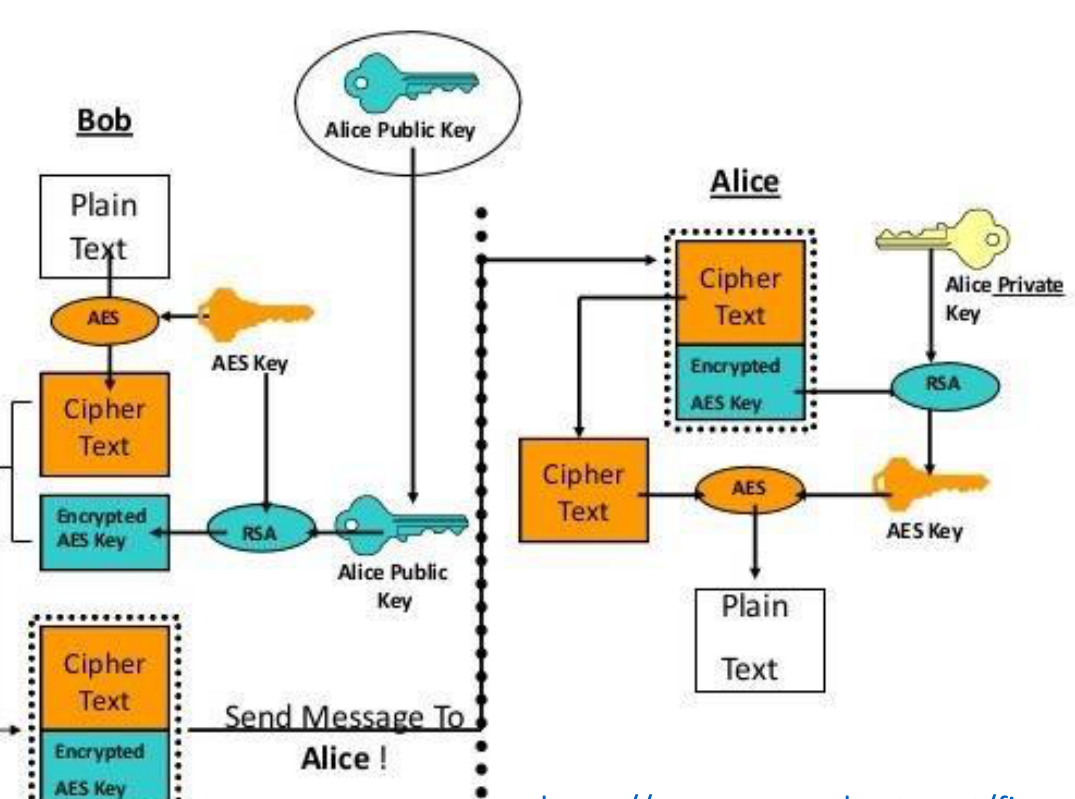
\includegraphics[width=117.60mm,height=219.78mm]{../../images/llm/page_006_img_01.png}%
\end{textblock*}

\end{document}
